In this chapter, we describe the geometry generation process central to the optimization framework. The generated geometry serves as the foundation for simulation using the lattice Boltzmann method described in Chapter \ref{lbm}. The geometry is directly influenced by optimization parameters that define it. The values of these parameters arise from the used optimization algorithm and are used to dynamically fill predefined geometry templates, ensuring that the model accurately represents the system under varying conditions. The templates are implemented in Gmsh -- a mesh generation software allowing parametric definition of geometries \cite{gmsh} -- hence the type of the file \texttt{.geo}.

The overview of the entire process is presented in Figure \ref{fig:meshgen overview}.


\begin{figure}[H]
	\centering
	\vspace{6mm}
	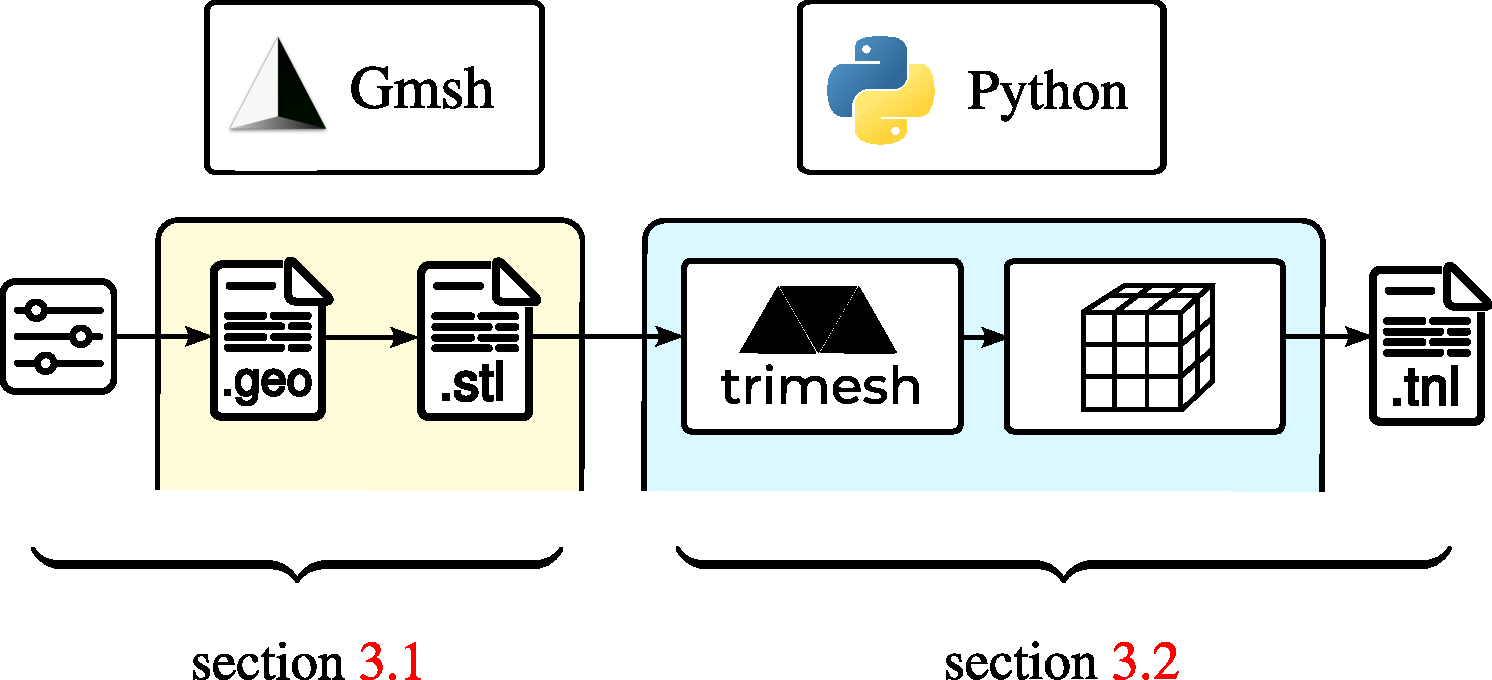
\includegraphics[width=.85\textwidth]{figures/meshgen.pdf}
	\vspace{4mm}
	\caption{Overview of the \texttt{meshgen} package.}
	\label{fig:meshgen overview}
\end{figure}
